\documentclass{standalone}
\usepackage{tikz}
\usetikzlibrary{shapes}
\usepackage{tikzpeople}

\begin{document}

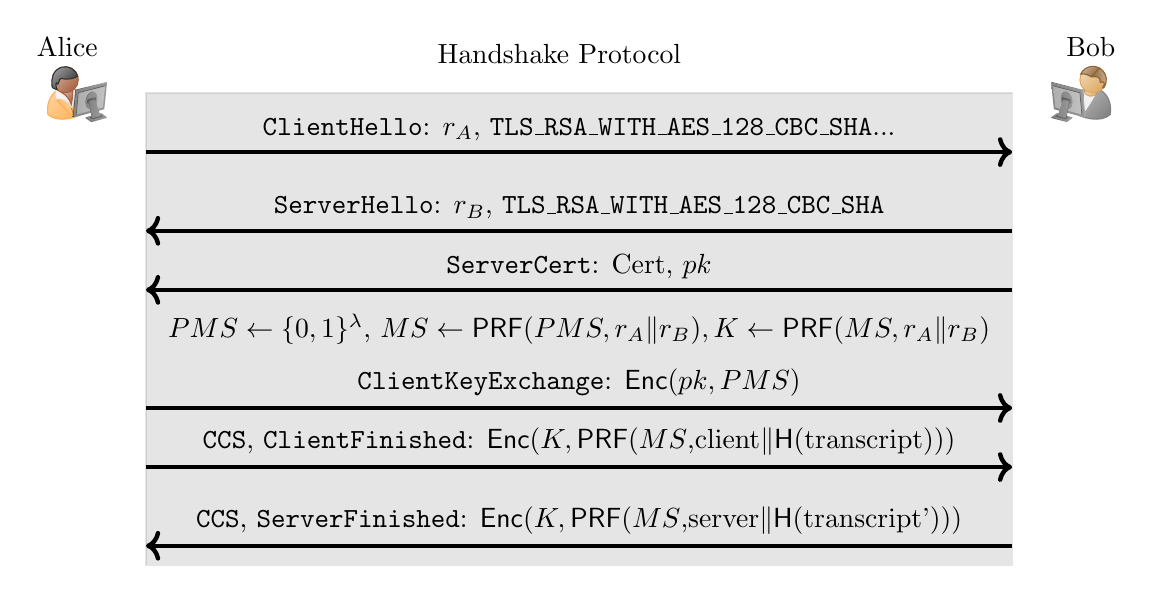
\begin{tikzpicture}
\tikzset{
	cylinder/.style={draw,
		shape=cylinder,
		name=nodename, % Can be defined arbitrarily
		alias=cyl, % Will be used by the ellipse to reference the cylinder
		aspect=1.5,
		minimum height=8.5cm,
		minimum width=2.25cm,
		color=blue,
		fill= blue!30,
		outer sep=-0.5\pgflinewidth, % to make sure the ellipse does not draw over the lines
		%shape border rotate=90
}}

\draw[draw=black,fill=black, opacity=0.1] (1,6) rectangle  (12,0);
\node[] (HSKLBL) at (6.25,6.5) {Handshake Protocol};
\node[alice, monitor, label=Alice, minimum size=0.5cm] (Alice) at (0,6) {};
\node[bob, mirrored, monitor, label=Bob, minimum size=0.5cm] (Bob) at (13,6) {};

{\draw[->, ultra thick] (1,5.25)  -- (12,5.25) node[midway, above] {\texttt{ClientHello}: $r_A$, \texttt{TLS\_RSA\_WITH\_AES\_128\_CBC\_SHA}...};}
{\draw[<-, ultra thick] (1,4.25)  -- (12,4.25) node[midway, above] {\texttt{ServerHello}: $r_B$, \texttt{TLS\_RSA\_WITH\_AES\_128\_CBC\_SHA}};}
{\draw[<-, ultra thick] (1,3.5)  -- (12,3.5) node[midway, above] {\texttt{ServerCert}: Cert, $pk$};}
{\node[] (PMS) at (6.5,3) {$PMS\gets \{0,1\}^{\lambda}$, $MS \gets \mathsf{PRF}(PMS,r_A\|r_B),K \gets \mathsf{PRF}(MS,r_A\|r_B)$};}
{\draw[->, ultra thick] (1,2)  -- (12,2) node[midway, above] {\texttt{ClientKeyExchange}: $\mathsf{Enc}(pk,PMS)$};}
{\draw[->, ultra thick] (1,1.25)  -- (12,1.25) node[midway, above] {\texttt{CCS}, \texttt{ClientFinished}: $\mathsf{Enc}(K,\mathsf{PRF}$($MS$,client$\|\mathsf{H}$(transcript)))};}
{\draw[<-, ultra thick] (1,0.25)  -- (12,0.25) node[midway, above] {\texttt{CCS}, \texttt{ServerFinished}: $\mathsf{Enc}(K, \mathsf{PRF}$($MS$,server$\|\mathsf{H}$(transcript')))};}
\end{tikzpicture}

\end{document}
